\documentclass[11pt]{article}

\usepackage[backgroundcolor=white,textsize=small,linecolor=red]{todonotes}

\usepackage[margin=30mm]{geometry}
\usepackage{natbib}


%--------------------
% Math
\usepackage[fleqn]{amsmath}
\usepackage{amsfonts}
\usepackage{amsthm}
\usepackage{amssymb}
\usepackage{stmaryrd}
\usepackage{multicol}
\usepackage{graphicx}

\newcommand{\mvalueof}[1]{\llbracket#1\rrbracket}
\newcommand{\citeposs}[2][]{\citeauthor{#2}'s (\citeyear[#1]{#2})}
\newcommand{\tuple}[1]{\ensuremath{\left\langle #1 \right\rangle}} 

\newcommand{\hloranj}[1]{\textcolor[rgb]{.8,.33,.0}{#1}}% prints in orange
\newcommand{\argmax}[1]{\underset{#1}{\operatorname{arg}\,\operatorname{max}}\;}
\newcommand{\argmin}[1]{\underset{#1}{\operatorname{arg}\,\operatorname{min}}\;}
\newcommand{\sbna}{\exists\lnot\forall}


%--------------------
%\usepackage{gb4e}
%
%\usepackage{setspace}
%\onehalfspacing
%
%\usepackage{soul} %underlining
%\setuldepth{a}




%\usepackage{inconsolata}

%-------------------


\title{Bounds, Semantics/Pragmatics-Divide, and Evolution}

\author{%\bf NAME1 and NAME2\\
    \today
}


\date{}

\begin{document}
\maketitle

\section{Short exposition}
The plan is to expand our work on the semantics/pragmatics divide by means of a (more extended) study on the lack of upper-bounds in the literal meaning of scalar expressions. The main idea of this extension, other than providing a more detailed treatment as well as a comparison with iterated learning, is to look at the effect multiple scalar pairs have on the dynamics. That is, we consider larger language fragments consisting of more than one pair of expressions of the ``some but not all'' vs. ``all''-form. 

\section{Differences to CogSci setup.}
\subparagraph{(I) Lexica and types.} $3$ pairs of scalar expressions. Each pair is a $(2,2)$-Boolean matrix, which means that a lexicon is now a $(8,8)$-matrix. We have two types of signaling behavior, literal and Gricean, and $6$ different $(2,2)$-lexica. The latter is the set of possible semantics of a single scalar pair. With three scalar pairs we have $6 \cdot 6 \cdot 6 = 216$ $(8,8)$-lexica. $216$ times two signaling behaviors makes for a total of $432$ types.

\subparagraph{(II) Observations.} Before, the set of all production observations was $O =$\linebreak  $\{\tuple{\tuple{s_1,m_i},\tuple{s_2,m_j}} | m_i, m_j \in M\}$. A member of $O$ encodes that a teacher produced $m_i$ in state $s_1$ and $m_j$ in $s_2$, i.e. it encodes one witnessed message for each state. A datum $d$ was a sequence of length $k$ of members of $O$. Learners witnessed such data sequences. Now, more in line with \citet{griffiths+kalish:2007}, $O = \{\tuple{s_i,m_j} | s_i \in S, m_j \in M\}$ and $d$ is a sequence of length $k$ of members of $O$. The main difference is that now some $d$ do not provide any production information for some states.

\subparagraph{(III) Computational load.} Computing the $Q$-matrix from the set of all observation sequences of length $k$ is computationally intractable for large $k$. Here, we follow \citet{griffiths+kalish:2007} as well in sampling $1000$ sequences $d$ from the set of all sequences when $k > 4$. We use this sampled subset to compute $Q$ instead of the full set of sequences\footnote{Thomas: Assuming this solves the problem. My computer can't handle the computation even with sampling but a better computer may. I'm still waiting on people from my project to address my request for computation time on our server.}
	      
\subparagraph{(IV) Mutation/Learning matrix.} If the results warrant it, classical (unweighted) learning instead of communal (weighted) learning.\footnote{Thomas: We can save the results for both cases in one go and decide on this later.}

\paragraph{Further modifications we may want to keep in mind (but currently don't make use of).}
\subparagraph{(I) Cost for pragmatic reasoning.} At least in the CogSci setup the effect of adding cost to pragmatic reasoning is unsurprising: High cost for pragmatic signaling lowers the prevalence of pragmatic types. Lexica that semantically encode an upper-bound benefit the most from this. However, the cost needed to be substantial to make the pragmatic English-like lexicon stop being the incumbent type (particularly when learning is communal). 

\subparagraph{(II) Negative learning bias.} Instead of penalizing complex semantics (semantic upper-bounds) one may consider penalizing simple semantics (no upper-bounds). This is useful as a sanity check but also yields unsurprising results in the CogSci setup: The more learners are biased against simple semantics, the more prevalent are lexica that semantically encode upper-bounds. 

\subparagraph{(III) Inductive bias.} A second learning bias that codifies the idea that lexica should be uniform, i.e. be biased towards either lexicalizing an upper-bound for all weaker alternatives in a scalar pair or for none.

\subparagraph{(IV)  Uncertainty.} The other advantage of non-upper bounded semantics lies in being non-committal to the negation of stronger alternatives when the speaker is uncertain. Adding this to the model requires the most changes to our present setup and some additional assumptions about the cues available to players to discern the speaker's knowledge about the state she is in. 

\section{General setup}
\subsection{Part 1: Signaling.}

We consider a population of players with two signaling strategies, literal and Gricean (level $0$ and $1$ below), each equipped with one of $216$ lexicons. This yields a total of $432$ distinct player types $t \in T$. However, each lexicon is composed of three independent lexical pairs. That is, while $|M| = |S| = 8$, we can decompose each lexicon into three independent $(2,2)$-matrices. A lexicon is a combination of three such matrices. These are listed in Table \ref{tab:lexica}. 

\begin{table}[h]
\centering 
\begin{tabular}{l c l}
$L_1$ = $\begin{pmatrix} 0 & 0 \\ 1 & 1 \end{pmatrix}$ & 
$L_2$ = $\begin{pmatrix} 1 & 1 \\ 0 & 0 \end{pmatrix}$ & 
$L_3$ = $\begin{pmatrix} 1 & 1 \\ 1 & 1 \end{pmatrix}$\\[0.5cm]

$L_4$ = $\begin{pmatrix} 0 & 1 \\ 1 & 0 \end{pmatrix}$ &
$L_5$ = $\begin{pmatrix} 0 & 1 \\ 1 & 1 \end{pmatrix}$ &
$L_6$ = $\begin{pmatrix} 1 & 1 \\ 1 & 0 \end{pmatrix}$
\end{tabular}
\caption{{\footnotesize Set of possible $(2,2)$-matrices, i.e. possible semantics for a pair of scalar expressions.}}
\label{tab:lexica}
\end{table}

As in the CogSci paper, $L_4$ (semantic upper-bound for $m_2$) and $L_5$ (no semantic upper-bound for $m_2$) are the target lexica. Gricean $L_5$ users can convey/infer the bound pragmatically, while literal/Gricean $L_4$ users do so semantically.

\paragraph{Signaling behavior.} With $\lambda \geq 1$ (rationality parameter), $\alpha \in [0,1]$ (pragmatic violations) and $pr \in \Delta(S)$ a common prior over $S$ (uniform so far):


\vspace{-0.15cm}
\begin{flalign}
&R_{0}(s|m;L) \propto pr(s) L_{sm}\label{litl}\\
&S_{0}(m|s;L) \propto \exp(\lambda \; L_{sm}) \label{lits}\\
&R_{1}(s|m;L) \propto pr(s) S_{0}(m|s;L) \label{pragl}\\
&S_{1}(m|s;L) \propto  \exp(\lambda \; R_{0}(s|m;L)^\alpha) \label{prags}
\end{flalign}


\paragraph{Symmetrized expected utility.} With $P \in \Delta(S)$ (uniform so far; therefore $P = pr$):
\begin{itemize}

  \item $U(t_i,t_j) = [U_S(t_i,t_j) + U_R(t_i,t_j)] / 2$
  \item $U_S(t_i,t_j) = \sum_s P(s) \; \sum_m P_S(m|s;t_i) \; \sum_{s'} P_R(s'|m,t_j) \; \delta(s,s')$, where $\delta(s,s')$ returns $1$ iff $s = s'$ and otherwise $0$
  \item $U_R(t_i,t_j) = U_S(t_j,t_i)$
\end{itemize}


\subsection{Part 2: Mutation \& replication.}
The proportion of players of type $i$, $x_i$, is initialized as an arbitrary distribution over $T$. $p^\star \in \Delta(T)$ is learning a prior over (player) types dependent only on the lexicon of the type. 
\begin{itemize}
    \item $f_i = \sum_j x_j U(x_i,x_j)$
    \item $\Phi = \sum_i x_i f_i$
    \item $Q_{ij} \propto \sum_d P(d|t_i) \; P(t_j|d)$, where $P(t_j|d) \propto p^\star(t_j) P(d|t_j)$ and $d$ is a sequence of observations of length $k$ of the form \tuple{\tuple{s_i,m_j}, ... \tuple{s_k, m_l}}.
\end{itemize}

\paragraph{Weighted (communal) learning vs. unweighted (parental) learning}

\begin{itemize}
	\item For parental learning (standard RMD): $\dot x_i = \sum_j Q_{ji} \frac{x_j f_j}{\Phi}$
	\item For communal learning (our variant in CogSci): $\dot x_i = \sum_j N_{ji} \frac{x_j f_j}{\Phi}$, where $N_{ji} = x'_{i} Q_{ji}$ and $x'_i$ is the proportion of type $i$ in the previous generation.
\end{itemize}

\subsection{Model parameters \& procedure} 
\begin{enumerate}
  \item Sequence length $k$
  \item Pragmatic production parameter $\alpha$
  \item Rationality parameter $\lambda$
  \item Learning prior over types (lexica); cost parameter $c$. $p^\star(t_i) \propto n - c \cdot r$ where $n$ is the total number of states and $r$ that of upper-bounded messages only true of $s_1$ in $t_i$'s lexicon (if only $s_1$ is true of a message, then this message encodes an upper-bound). Then the score for $L_1$, $L_3$, $L_5$ is $2$, that of $L_4$ and $L_6$ is $2-c$, and that of $L_2$ is $2-2c$; Normalization over lexica scores yields the prior over lexica (which is equal to the prior over types).   
  \item Prior over meanings ($pr$). We assume that $pr(s) = \frac{1}{|S|}$ for all $s$.
  \item True state distribution ($P$). We currently assume that $P = \frac{1}{|S|}$ but it may be interesting to vary this
\end{enumerate}



\paragraph{Procedural description.} The game is initialized with some arbitrary distribution over player types. At the game's onset we compute $Q$ once based on the set of sequences $D$. If $k > 4$, $1000$ sequences are sampled from $D$ and used to compute $Q$ (instead of the full set). Replicator dynamics are computed based on the fitness of each type in the current population as usual. In the case of community learning, $Q$ is weighted by the previous population vector in each new generation.

\paragraph{Presentation.} We have a large number of types, some of which are highly similar. For instance, a type that uses $L_4$, $L_5$ and $L_4$ for her respective three scalar pairs is a different type than one that uses $L_5$, $L_4$ and $L_4$. As our goal is to elucidate the role and prevalence of upper-bounds, we may summarize the results not by type but by lexica counts. For instance, if the previous two types where all we had this would mean that $L_4$'s proportion is roughly $.66$ and $L_5$'s $.33$ (irrespective of signaling behavior). An example is given below for communal learning with a single scalar pair against three scalar pairs ($\alpha = 1, c = .7, \lambda = 30, k = 3$):


\begin{figure}[h] %htb for exact position
	\centering
	\resizebox{13cm}{!}{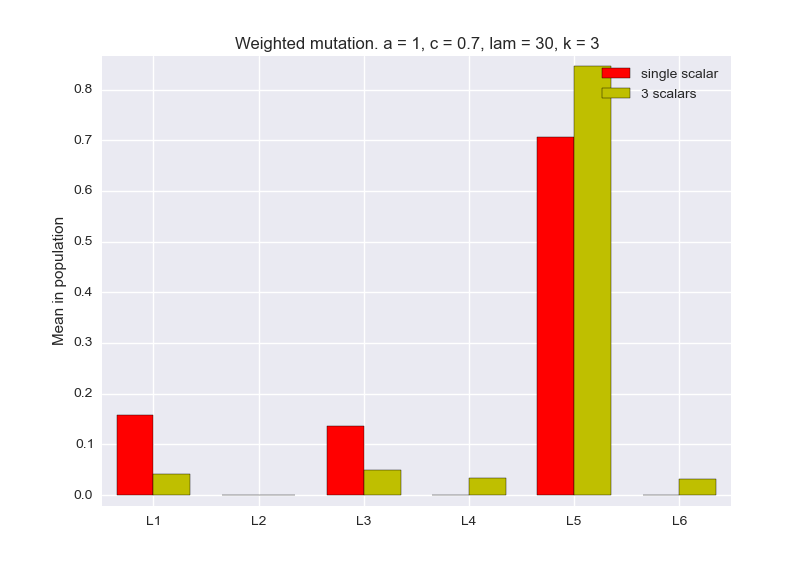
\includegraphics{../plots/wgh-single-vs-multi-k3-c70}}
\end{figure}


%\bibliographystyle{apacite}
\bibliographystyle{unsrtnat}

%\setlength{\bibleftmargin}{.125in}
%\setlength{\bibindent}{-\bibleftmargin}
\bibliography{./bounds-rmd}


\end{document}
